\documentclass[25pt, a0paper,
               colspace=15mm, subcolspace=0mm,
               blockverticalspace=17mm]{tikzposter} % See Section 

\usepackage{graal-poster}
\usepackage{array}
\usepackage{multirow}
\usepackage{multicol}
%\usepackage{fontspec}

%\usepackage[font=small,labelfont=bf]{caption} % Required for specifying captions to tables and figures



\definecolor{PaleBlue}{rgb}{0,.55,.9}
\definecolor{PaleGreen}{rgb}{0,.7,.25}
\definecolor{RedPink}{rgb}{.9,0,.2}
\definecolor{Pink}{rgb}{.85,.35,.7}
\definecolor{Purple}{rgb}{.6,0,.75}
\definecolor{Orange}{rgb}{.9,.3,.05}

\colorlet{attentionColor}{Orange}
\colorlet{charEmbedColor}{RedPink}
\colorlet{predEmbedColor}{Pink}


\def\pathwidth{2pt}
\def\nodewidth{3pt}
\def\cornerCurvature{7pt}

\tikzstyle{embed}=[%
  draw,
  #1,
  % line width=3pt,
  anchor=north,
  minimum width=.8cm,
  minimum height=1.6cm,
  inner sep=0pt,
  text=#1!65!black,
  font=\fontsize{25pt}{24}\selectfont,
  ]


\title{\parbox{\linewidth}{\centering Reconnaissance de dessins manuscrits avec jeu de données Quick, Draw!}}
\institute{Département d'informatique et de génie logiciel, Université Laval}
\author{William Bourget, Samuel Lévesque}


\begin{document}
\maketitle



\begin{columns}
\column{.4}
\block{Introduction}{

Nous souhaitons livrer un produit utilisable en temps réel par l'entremise de ce projet. 
Les projets académiques habituellement réalisés se concentrent sur les l'optimisatione et la comparaison de modèles, mais nous n'avons jamais eu la chance de terminer la chaîne d'un projet et d'utiliser les prédictions des modèles développés en \colorbold{temps réel}.

\vspace{5mm}
\textbf{Motivations:}
\begin{itemize}
  \item Application des techniques de \colorbold{traitement d'images} à partir d'un grand corpus de données.
  \item Déploiement complet d'un modèle prédictif pour usage par des non-experts.
\end{itemize}

\vspace{0mm}
\textbf{Buts:}
\begin{itemize}
  \item Apprendre à traiter efficacement de grandes quantités de données.
  \item Se familiariser avec les outils d'\colorbold{infonuagique} des grands joueurs pour projets à grande échelle.
  \item Développer une \colorbold{interface graphique} permettant à des usagers de tester notre modèle en temps réel.
  \item Couvrir l'ensemble de la chaîne d'un projet en intelligence artificielle du traitement des données à l'utilisation du modèle dans un contexte de vie réelle.
\end{itemize}

}


\column{0.6}
\block{Structure du réseau et méthodologie}{

\vspace{-15pt}
% Comick v3.0 (TheFinalComick)
\begin{center}
\begin{tikzpicture}[
          scale=1.5,
          lstm_right/.style={draw, minimum width=1cm, minimum height=.5cm, inner sep=0pt, anchor=north, PaleGreen},
          lstm_left/.style={draw, minimum width=1cm, minimum height=.5cm, inner sep=0pt, PaleBlue},
          every path/.style={line width=\pathwidth},
          every node/.append style={line width=\nodewidth}]
  \def\w{1cm}
  \def\h{2cm}
  \def\y{-.2}
  \def\scalespacetoken{1.5}
  \def\scalespacecontext{2}
  \def\oplstmdist{-1}
  \def\wordToEmbed{-5mm}
  \def\embedToLstm{-7mm}
  \def\whiteLineWidth{15pt}

  % \draw (-6,\y) -- (10,\y);
  % Char embedding
  \foreach \letter [count=\i] in {S, a, l, e, m}{
    \pgfmathsetmacro\pos{\i-1}
    \node[anchor=mid, inner sep=0](\letter) at (\scalespacetoken*\pos,0) {\letter};
    \node[embed=charEmbedColor](\letter _embed) at (\scalespacetoken*\pos,\wordToEmbed){c};
    \node[lstm_left](\letter _lstm_left) at ([yshift=\embedToLstm]\letter _embed.south) {};
    \node[lstm_right](\letter _lstm_right) at (\letter _lstm_left.south) {};

    \draw[-mytip] (\letter _embed) -- (\letter _lstm_left);
  };

  \draw[decorate,decoration={brace,amplitude=.6cm}]
    ([yshift=1pt,xshift=-.15cm]S.north west) -- node[midway, yshift=12mm]{Unknown word} ([yshift=1pt,xshift=.15cm]m.north east);

  % LSTM arrows
  \foreach \a/\b in {S/a, a/l, l/e, e/m}{
    \draw[mytip-, PaleBlue] (\a _lstm_left) -- (\b _lstm_left);
    \draw[-mytip, PaleGreen] (\a _lstm_right) -- (\b _lstm_right);
  };

  \node[operator](cat_word) at ([yshift=\oplstmdist cm]l_lstm_right.south) {\large $\|$};
  \draw[-mytip, rounded corners=\cornerCurvature, PaleBlue] (S_lstm_left.west) -| +(-.5,-.65) |- (cat_word);
  \draw[-mytip, rounded corners=\cornerCurvature, PaleGreen] (m_lstm_right.east) -| +(.3,-.43) |- (cat_word);

  % Left side
  \def\leftcontdist{-.5*\scalespacecontext}
  \foreach \word [count=\i] in {goalkeeper, which, goal, Syrian}{
    \pgfmathsetmacro\pos{-\scalespacecontext*\i+\leftcontdist}
    \node[anchor=mid, inner sep=0, baseline=0](\word) at (\pos,0) {\word};
    \node[embed=Purple](\word _embed) at (\pos,\wordToEmbed){w};
    \node[lstm_left](\word _lstm_left) at ([yshift=\embedToLstm]\word _embed.south) {};
    \node[lstm_right](\word _lstm_right) at (\word _lstm_left.south) {};

    \draw[-mytip] (\word _embed) -- (\word _lstm_left);
  };

  \foreach \a/\b in {Syrian/goal, goal/which, which/goalkeeper}{
    \draw[mytip-, PaleBlue] (\a _lstm_left) -- (\b _lstm_left);
    \draw[-mytip, PaleGreen] (\a _lstm_right) -- (\b _lstm_right);
  };

  \def\opdist{-2.2}

  \path (Syrian_lstm_right.south west) -- (goalkeeper_lstm_right.south east) node[midway, operator, yshift=\opdist cm](cat_left) {\large $\|$};

  \draw[-mytip, rounded corners=\cornerCurvature, PaleBlue] (Syrian_lstm_left.west) -| +(-.5,-.65) |- (cat_left);
  \draw[-mytip, rounded corners=\cornerCurvature, PaleGreen] (goalkeeper_lstm_right.east) -| +(.3,-.43) |- (cat_left);
  
  \draw[decorate,decoration={brace,amplitude=.6cm}]
    ([yshift=1pt,xshift=-.15cm]Syrian.north west) -- node[midway, yshift=12mm]{Left context} ([yshift=1pt,xshift=.15cm]goalkeeper.north east);

  % Right side
  \def\rightcontdist{3.5*\scalespacecontext}
  \foreach \word/\tag [count=\i] in {Bitar, appeared, to, have}{
    \pgfmathsetmacro\pos{\scalespacecontext*\i+\rightcontdist}
    \node[anchor=mid, inner sep=0, baseline=0](\word) at (\pos,0) {\word};
    \node[embed=Purple](\word _embed) at (\pos,\wordToEmbed){w};
    \node[lstm_left](\word _lstm_left) at ([yshift=\embedToLstm]\word _embed.south) {};
    \node[lstm_right](\word _lstm_right) at (\word _lstm_left.south) {};

    \draw[-mytip] (\word _embed) -- (\word _lstm_left);
  };

  \foreach \a/\b in {Bitar/appeared, appeared/to, to/have}{
    \draw[mytip-, PaleBlue] (\a _lstm_left) -- (\b _lstm_left);
    \draw[-mytip, PaleGreen] (\a _lstm_right) -- (\b _lstm_right);
  };

  \draw[decorate,decoration={brace,amplitude=.6cm}]
    ([yshift=1pt,xshift=-.15cm]Bitar.north west) -- node[midway, yshift=12mm]{Right context} ([yshift=1pt,xshift=.15cm]have.north east);

  \def\decalage{-.0}
  \pgfmathsetmacro\opdistright{\opdist + \decalage}
  \path (Bitar_lstm_right.south west) -- (have_lstm_right.south east) node[midway, operator, yshift=\opdistright cm](cat_right) {\large $\|$};

  \coordinate(mid) at ([yshift=.38cm]cat_right.north);
  \draw[-mytip, rounded corners=\cornerCurvature, PaleGreen] (have_lstm_right.east) -| ++(.3,-.25) %node[fill]{}
  |- ([yshift=-.15cm]mid) %node[fill]{}
  -| ++(-2,-.3) %node[fill]{}
  |- (cat_right);

  \path (Bitar_lstm_left.west)
  -| ++(-.5,-.33) coordinate(p1)
  |- ([yshift=.15cm]mid) coordinate(p2)
  -| ++(2,-.4) coordinate(p3)
  |- (cat_right);
  \draw[white, line width=\whiteLineWidth] (p2) -| (p3);
  \draw[-mytip, rounded corners=\cornerCurvature, PaleBlue] (Bitar_lstm_left.west)
  -| (p1)
  |- (p2)
  -| (p3)
  |- (cat_right);
  

  % Head
  \def\fcdist{-.5}
  \pgfmathsetmacro\fcdistleft{\decalage + \fcdist}
  % FCs
  \draw[-mytip] (cat_left.south) -- ++(0,\fcdistleft) node[draw, anchor=north, rectangle split, rectangle split parts=2](fc_left) {Fully connected \nodepart{second} tanh};
  \draw[-mytip] (cat_right.south) -- ++(0,\fcdist) node[draw, anchor=north, rectangle split, rectangle split parts=2](fc_right) {Fully connected \nodepart{second} tanh};
  \draw[-mytip] (cat_word.south) -- ++(0,\fcdist) node[draw, anchor=north, rectangle split, rectangle split parts=2](fc_word) {Fully connected \nodepart{second} tanh};

  % Attention module
  \path ([yshift=2*\fcdist cm]fc_word.south west) -| node[pos=.25, operator, anchor=north, attentionColor](cat_att) {\Large $\|$} (fc_left.east);
  \draw[-mytip, rounded corners=\cornerCurvature, attentionColor] (fc_word.south) |- ++(2*\fcdist,1*\fcdist) -| (cat_att.north);
  \draw[-mytip, attentionColor] (cat_att.south) -- ++(0,\fcdist) node[draw, anchor=north, rectangle split, rectangle split parts=2, text=attentionColor!60!black](fc_att) {Fully connected \nodepart{second} softmax};

  \draw[-mytip, rounded corners=\cornerCurvature, attentionColor] (fc_left.south) |- (cat_att);
  \draw[-mytip, rounded corners=\cornerCurvature, attentionColor] (fc_right.south) |- (cat_att);

  \def\softmaxShift{-.5}
  % Ponderation
  \path ([yshift=\softmaxShift cm]fc_att.west) -| node[attentionColor, midway, operator](pond_left) {\Large $\times$} (fc_left);
  \draw[-mytip, attentionColor] ([yshift=\softmaxShift cm]fc_att.west) -- (pond_left);
  \draw[-mytip] (fc_left) -- (pond_left);
  
  \path ([yshift=\softmaxShift cm]fc_att.east) -| node[attentionColor, midway, operator](pond_right) {\Large $\times$} (fc_right);
  \draw[-mytip, attentionColor] ([yshift=\softmaxShift cm]fc_att.east) -- (pond_right);
  \draw[-mytip] (fc_right) -- (pond_right);

  \path ([yshift=1.5*\fcdist cm]fc_att.south) -| node[attentionColor, midway, operator](pond_word) {\Large $\times$} (fc_word);
  \draw[-mytip, attentionColor, rounded corners=\cornerCurvature] (fc_att.south) |- (pond_word);

  \draw[white, line width=\whiteLineWidth] ([yshift=2*\fcdist cm]fc_word.south) -- ([yshift=.5*\fcdist cm]pond_word);
  \draw[-mytip] (fc_word) -- (pond_word);


  % End
  \draw[-mytip] (pond_word.south) -- ++(0,\fcdist) node[anchor=north, operator](plus) {\large $+$};
  \draw[-mytip, rounded corners=\cornerCurvature] (pond_left) |- (plus);
  \draw[-mytip, rounded corners=\cornerCurvature] (pond_right) |- (plus);


  \node[draw, anchor=north](tanh-fc1) at ([yshift=\fcdist cm]plus.south) {Fully connected};

  \node[draw, predEmbedColor, text=predEmbedColor!40!black, anchor=north] (output) at ([yshift=\fcdist cm]tanh-fc1.south) {Predicted embedding};
  \draw[-mytip] (plus) -- (tanh-fc1);
  \draw[-mytip] (tanh-fc1) -- (output);


  % Legend
  \begin{scope}[xshift=14cm, yshift=-9.5cm,
          every path/.style={line width=\pathwidth},
          every node/.append style={line width=\nodewidth}]
  \def\legspace{-1.3}
  \def\h{1.3cm}
  % First col
  \node[embed=charEmbedColor, anchor=center, minimum height=\h, minimum width=.8cm](leg char embed) at (0,0*\legspace) {c};
  \node[anchor=west] at (.5,0*\legspace) {Character embedding};

  \node[embed=Purple, anchor=center, minimum height=\h, minimum width=.8cm](leg word embed) at (0,1*\legspace) {w};
  \node[anchor=west] at (.5,1*\legspace) {Word embedding};

  \node[draw, PaleBlue, minimum width=1cm, inner sep=0pt, minimum height=.5cm, anchor=south] (leg lstm left) at (0,2*\legspace) {};
  \node[draw, PaleGreen, minimum width=1cm, inner sep=0pt, minimum height=.5cm, anchor=north] (leg lstm right) at (leg lstm left.south) {};
  \node[anchor=west] at (.5,2*\legspace) {Bidirectional LSTM};

  \node[operator, minimum size=14mm](leg cat) at (0,3*\legspace) {$\|$};
  \node[anchor=west] at (.5,3*\legspace) {Concatenation};

  \node[operator, minimum size=14mm](leg plus) at (0,4*\legspace) {$+$};
  \node[anchor=west, align=left] at (.5,4*\legspace) {Element-wise\\[-3pt] summation};

  \node[operator, minimum size=14mm](leg mult) at (0,5*\legspace) {$\times$};
  \node[anchor=west, align=left] at (.5,5*\legspace) {Multiplication\\[-3pt] by a constant};

  \draw[attentionColor, line width=4pt] (-.35, 6*\legspace) -- (.35, 6*\legspace);
  \node[anchor=west, align=left] at (.5, 6*\legspace) {Attention module};
  \end{scope}

\end{tikzpicture}
\end{center}

The net consists in 3 bi-LSTM taking as input the left context, the right context and the word characters. An attention module ponderates their outputs which are then combined in a last fully connected layer.


}
\end{columns}




\begin{columns}
\column{.4}
\block[bodyoffsety=0mm, titleoffsety=0mm]{Contraintes}{

Plusieurs contraintes dans la réalisation de ce projet nous ont empêchés de tester toutes les avenues que nous avions initialement envisagées.
\colorbold{Contraintes computationnelles:}
\begin{itemize}
  \item \textbf{Enjeux de mémoire:}
	  \begin{itemize}
	      \item Incapacité à charger l'ensemble du jeu de données en \colorbold{mémoire}.
	      \item Conservation des images en \colorbold{format vectoriel} pour limiter l'espace de stockage nécessaire.
	  \end{itemize}
  \item \textbf{Enjeux de performance:}
	  \begin{itemize}
		\item Temps de traitement très important nous limite dans le nombre de modèles et de jeux d'hyperparamètres qu'on peut tester.
		\item Impossibilité d'entraîner les modèles sur nos postes personnels. Nous devons utiliser des solutions d'\colorbold{infonuagique} qui peuvent être coûteuses et complexes à utiliser avec un jeu de données aussi important.
	\end{itemize}
\end{itemize}

\textbf{Contraintes de l'interface graphique:}
\begin{itemize}
    \item Perte de l'\colorbold{information temporelle} des images vectorielles.
    \item Impossibilité d'utiliser \colorbold{différents canaux} pour simuler l'évolution temporelle du dessin.
	\item Perte de la séparation du dessin par trait.
\end{itemize}

\vspace{-.25mm}

}


\column{.6}
\block[bodyoffsety=0mm, titleoffsety=0mm]{Transformations}{





\vspace{-2mm}



%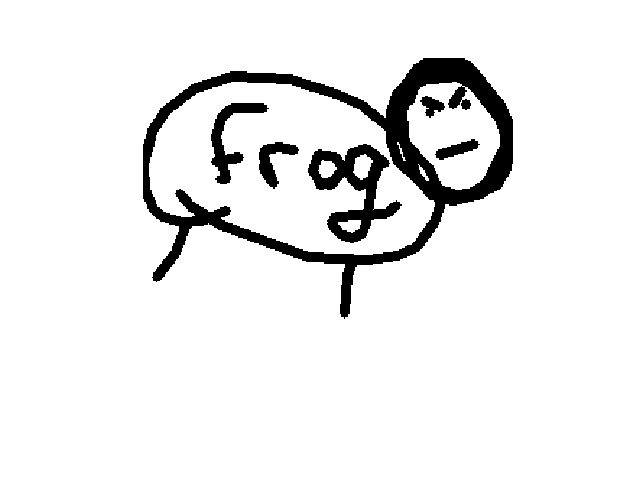
\includegraphics[width=0.5\textwidth]{figures/frog_draw_2.png}
%test texte

\begin{center}
Transformation de vecteurs de traits de crayon (position x, y)  en photos.
\end{center}

\begin{center}

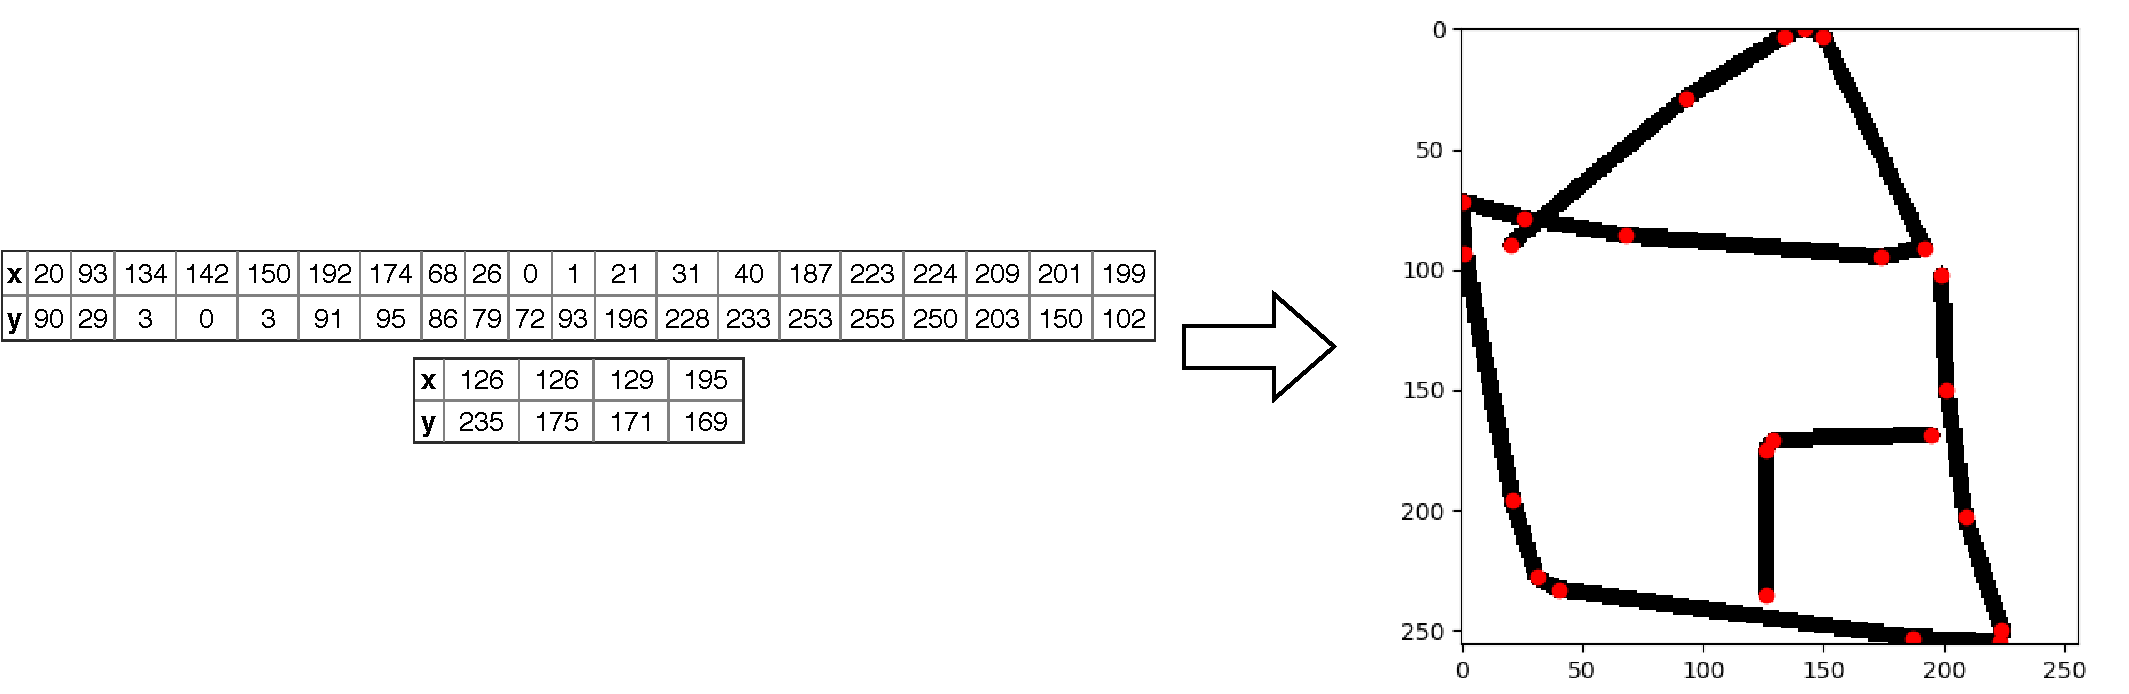
\includegraphics[width=44cm,height=44cm,keepaspectratio]{figures/Transformations_horizontal.pdf}

%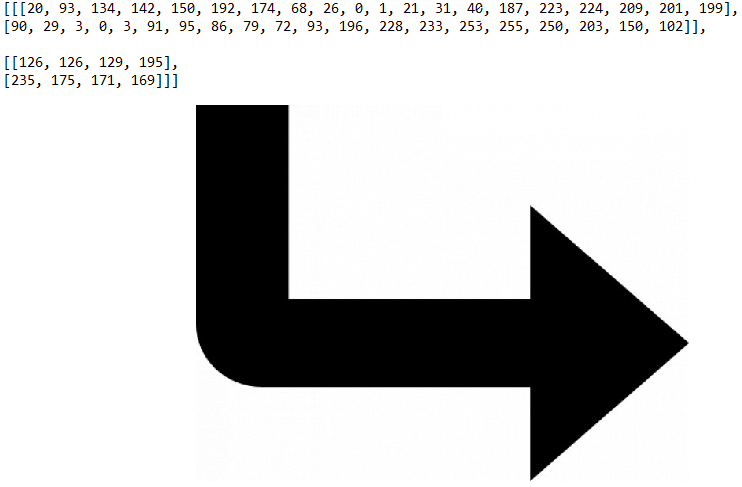
\includegraphics[width=15cm,height=15cm,keepaspectratio]{figures/vecteur_fleche.png}
%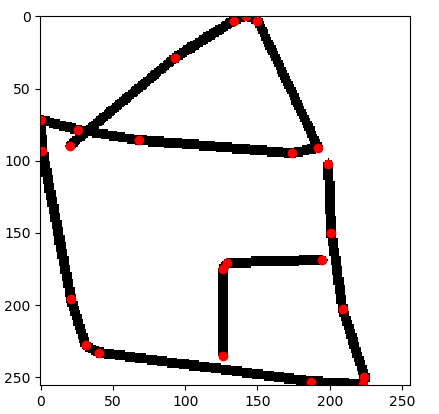
\includegraphics[width=15cm,height=15cm,keepaspectratio]{figures/housedraw.png}
%\captionof{figure}{Transformation des vecteurs }
\end{center}




\vspace{4mm}




\centering
\begin{itemize}
\item Images très différentes pour une même classe
\item Certaines images incomplètes
\end{itemize}

\vspace{4mm}
\begin{center}
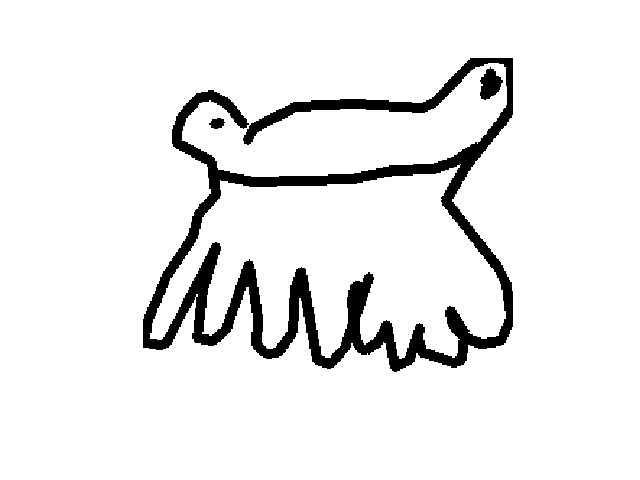
\includegraphics[width=9cm,height=9cm,keepaspectratio]{figures/frog_draw_1.png}
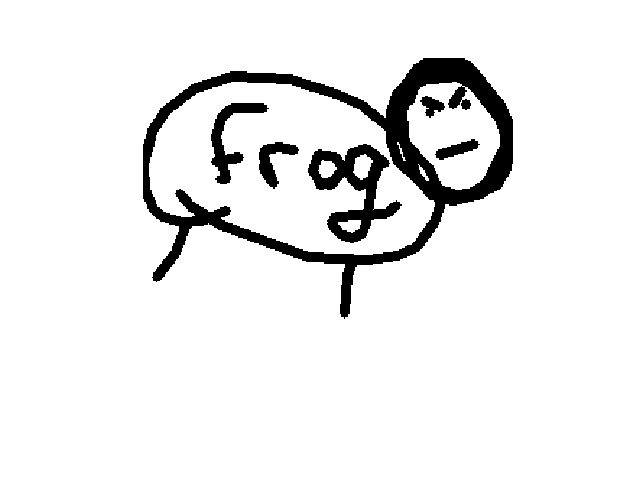
\includegraphics[width=9cm,height=9cm,keepaspectratio]{figures/frog_draw_2.png}

\includegraphics[width=9cm,height=9cm,keepaspectratio]{figures/frog_draw_3.png}

\includegraphics[width=9cm,height=9cm,keepaspectratio]{figures/frog_draw_4.png}


\end{center}






























}

\end{columns}




\begin{columns}

\column{.3}
\block{Description des données}{

Le jeu de données de Quick, Draw! est un sous-échantillon du jeu de données de Google AI contenant plus d'un milliard d'images. Voici quelques caractéristiques du jeu de données utilisé pour l'entraînement du modèle:

\begin{itemize}
	\item Jeux de données bruts et simplifiés disponibles (le jeu de données simplifié élimine des points inutiles qui se trouvent sur une même droite).
	\item \colorbold{345 classes}.
	\item \colorbold{$\approx$ 150 000 images/classe}.
	\item \colorbold{24,4 Gb} de données compressées en format .csv.
\end{itemize}

Utilisation des données compressées pour le projet pour limiter les enjeux de mémoire autant que possible sous hypothèse que les performances du modèle n'en souffriraient pas.

\vspace{-.5mm}

}


\column{.3}
\block{Performances}
{

\begin{center}
\setlength{\tabcolsep}{5mm}
\begin{tabular}{c c c c c c}
\toprule
\multirow{2}{*}{\textbf{Task}} & \multirow{2}{*}{\textbf{Tag}} & \multirow{2}{*}{\textbf{Ex.}} & \multicolumn{3}{c}{\textbf{Ponderation}}\\
\cline{4-6}
\addlinespace[3mm]
& & & Word & Left & Right\\
\midrule
\multirow{9}{*}{NER} & O           & 1039  & \colorbold{0.81}    & 0.08    & 0.11 \\
& B-PERS      & 63    & 0.21    & 0.31    & \colorbold{0.49} \\
& I-PER     & 119   & 0.16  & \colorbold{0.52} & 0.32 \\
& B-ORG     & 40  & 0.26  & 0.30  & \colorbold{0.44} \\ 
& I-ORG     & 3     & 0.27  & 0.31      & \colorbold{0.42} \\
& B-LOC     & 13  & 0.23      & 0.30  & \colorbold{0.47} \\
& I-LOC     & 2     & 0.16  & \colorbold{0.48} & 0.36 \\
& B-MISC      & 47  & \colorbold{0.40} & 0.21  & 0.39 \\
& I-MISC      & 5     & \colorbold{0.41} & 0.26  & 0.33 \\
\midrule
\multirow{5}{*}{POS} & NNP  & 308 & 0.29  & 0.31  & \colorbold{0.40} \\
& NN  & 46  & \colorbold{0.45} & 0.20  & 0.35 \\
& CD  & 827 & \colorbold{0.86} & 0.05  & 0.09 \\
& NNS & 23  & \colorbold{0.37} & 0.24  & \colorbold{0.39} \\
& JJ  & 100 & \colorbold{0.49} & 0.15  & 0.36 \\
\bottomrule
\end{tabular}
\end{center}

\vspace{1.5mm}
Average weights assigned to word's characters, left context and right context by the attention mechanism. We can clearly see the shift of attention according to the target entity. We also observe that the attention depends on the task at hand.
\vspace{-3mm}

}


\column{.4}
%\block{Autre section}
%{
%
%\begin{center}
\setlength{\tabcolsep}{5mm}
\begin{tabular}{c c c c c}
\toprule
\textbf{Task} & \textbf{Metric} & \textbf{Random Emb.} & \textbf{Our module} & \textbf{Gain}\\
\midrule
NER      & F1   & 77.56 & \colorbold{80.62} & 3.9\% \\
POS      & acc. & 91.41 & \colorbold{92.58} & 1.2\% \\
% Chunking & acc. & 92.63 & 93.16  & \textbf{93.19} \\
% Keyphrase& F1   & 37.40 & 39.56 & \textbf{39.77} \\
\bottomrule
\end{tabular}
\end{center}

\vspace{2.5mm}
The impact of our model on two NLP downstream tasks. We compare our OOV embeddings prediction scheme against random embeddings.
\vspace{-12mm}
%
%}


\block{Conclusion}{

\textbf{Discussion:}
\begin{itemize}
    \item Gains de performance avec notre méthode d'\colorbold{échantillonnage ciblé.}
    \item Réalisation \colorbold{\emph{end-to-end}} d'un projet d'analyse prédictive.
    Organisation du travail permettant le traitement de très \colorbold{grandes quantités de données}.
\end{itemize}

\textbf{Améliorations:}
\begin{itemize}
    \item  Utiliser différents \colorbold{canaux} d'images pour simuler l'évolution temporelle des dessins.
    \item Modification de l'interface graphique pour capter la composante temporelle des dessins avec séparation en traits.
    \item Utilisation de modèles moins corrélés dans le \colorbold{modèle par ensemble} (Autres architectures de réseaux profonds et autres modèles prédictifs).
\end{itemize}
\vspace{-3.5mm}

}
\end{columns}

\end{document}
